% Gere o PDF com o comando pdflatex, e o SVG com o comando
%
%  $ inkscape -l fig.svg source.tex
\documentclass{standalone}
\usepackage{tikz}
\usetikzlibrary{shapes}

\begin{document}

    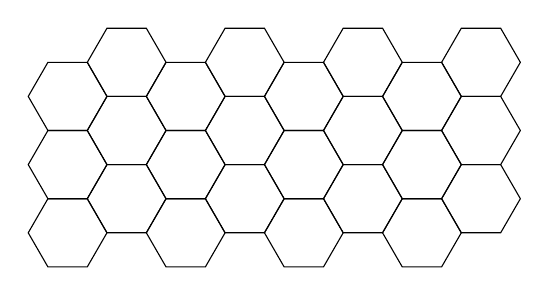
\begin{tikzpicture} [hexa/.style= {shape=regular polygon,
                                   regular polygon sides=6,
                                   minimum size=1cm, draw,
                                   inner sep=0,anchor=south}]

    \foreach \j in {0,...,7}{
        \ifodd\j 
             \foreach \i in {0,...,2}{\node[hexa] (h\j;\i) at ({\j/2+\j/4},{(\i+1/2)*sin(60)}) {};}        
        \else
             \foreach \i in {0,...,2}{\node[hexa] (h\j;\i) at ({\j/2+\j/4},{\i*sin(60)}) {};}
        \fi
    }

    \end{tikzpicture}

\end{document}
